%%%%%%%%%%%%%%%%%%%%%%%%%%%%%%%%%%%%%%%%%%%%%%%%%%%
% physicsresults.tex
%%%%%%%%%%%%%%%%%%%%%%%%%%%%%%%%%%%%%%%%%%%%%%%%%%%
\label{sec:physresult}
\subsection{\textbf{Results}}
A critical test of a physics list and the models and cross sections that 
comprise it is the comparison of its predictions to data from the calorimeters
of high energy physics experiments.  For this, \Gfour{} has relied upon test
beam data from the ATLAS \cite{bib:ATLAS}, CALICE \cite{bib:Calice}, and CMS
\cite{bib:CMS} collaborations.  The experimental parameters of interest include
the longitudinal, transverse and time distributions of shower energy, the 
visible deposited energy and energy resolution of the shower, and the relative 
importance of electromagnetic and hadronic energy as measured by the e/pi ratio.  

The latter parameter was the first for which good agreement between test beam 
data and a \Gfour{} physics list was obtained \cite{bib:generalpaper2}.  Since 
then, model improvement guided by thin target validation has resulted in good 
agreement in almost all the parameters mentioned above.  Discussed here are 
recent comparisons of predictions from the FTFP\_BERT physics list to test beam 
measurements of the longitudinal and transverse shower shapes, and the shower 
energy resolution.

In order to perform some of these comparisons a \Gfour{} geometry was developed 
which reproduced the essential details of the calorimeters used to take the 
data, while omitting other, less critical, yet time-consuming details.  Within
\Gfour{} this is referred to as the simplified calorimeter~\cite{6154433}.  Other
comparisons were performed within the various experiment collaborations using 
their own \Gfour{} geometry descriptions.

\begin{figure}[htb]
 \begin{center}
    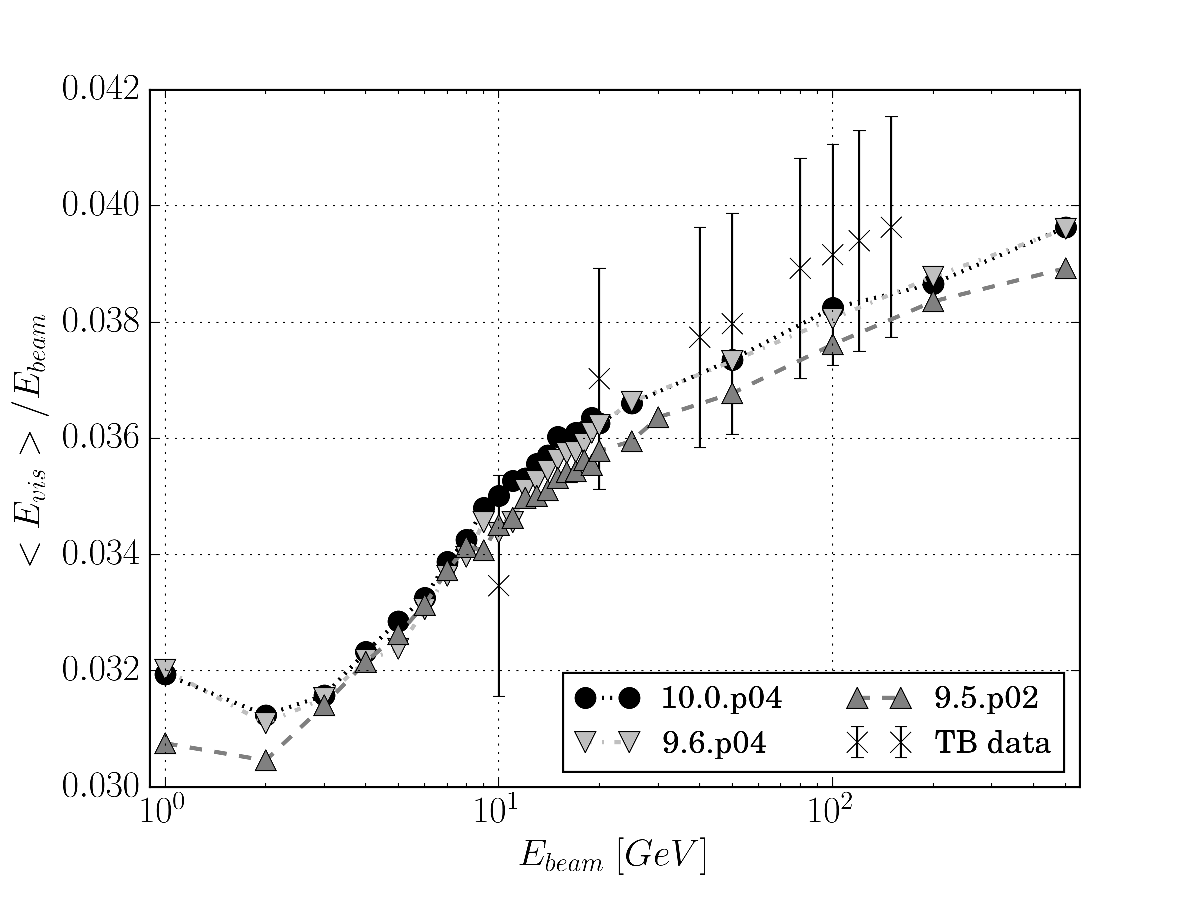
\includegraphics[width=0.5\textwidth]{figures/response.pdf}
    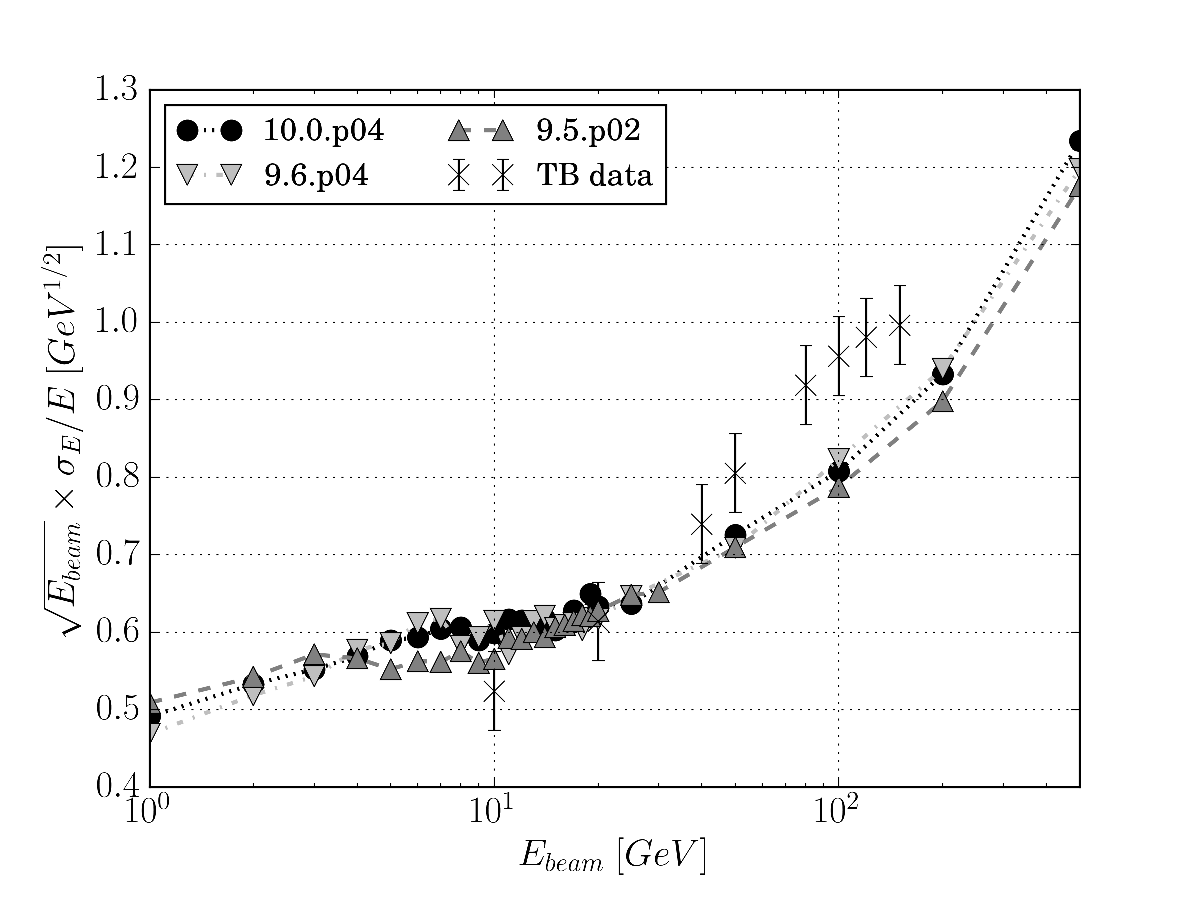
\includegraphics[width=0.5\textwidth]{figures/resolution.pdf}
   \caption{Comparison of recent \Gfour{} versions with test beam data for the
            response (top) and resolution (bottom) of the copper/liquid argon
            simplified calorimeter (ATLAS HEC).}
   \label{fig:response}
 \end{center}
\end{figure}

\subsubsection{Electromagnetic showers}
Significant efforts have been made to improve the simulation of electromagnetic
shower shapes in order to describe the details of the 
$H \rightarrow \gamma\gamma$ signal~\cite{Aad20121,Chatrchyan201230} and other 
reactions.  The bremsstrahlung process and the simulation of multiple scattering
were reviewed and improved, having been identified as key components in defining
shower shapes.  Calorimeters are particularly sensitive to the simulation of 
electron and gamma transport in the MeV energy region.  Therefore a large amount
of validation and benchmarking was, and continues to be, carried out for medium
and low energy electrons and gammas down to about 1 keV.  For these validation 
studies data from numerous thin-target and calorimeter test-beam experiments are 
used as well as comparisons with other \Gfour{} low energy electromagnetic 
models, such as the Livermore and Penelope sub-packages, which have been 
recently adapted to a common interface (see section \ref{sec:emuni}) with the 
standard electromagnetic sub-packages~\cite{pnst-VI}.

The process of multiple scattering (MSC) of charged particles is a key component
of Monte Carlo transport codes.  At high energy it defines the deviation of 
charged particles from ideal tracks, limiting the spatial resolution of 
detectors.  The scattering of low energy electrons defines the energy flow via 
volume boundaries.  This affects the sharing of energy between absorbers and 
sensitive elements, directly affecting shower shapes.  A comprehensive 
description of recent improvements of the \Gfour{} electromagnetic module can be
found in~\cite{1742-6596-396-2-022013}.
%  The general 
Good agreement was found when \Gfour{} predictions were compared with 
experimental data collected at the LHC
% is below the percent 
%level for energy response 
~\cite{1748-0221-6-04-P04001}.
% , and at the few percent 
% level for energy resolution and shower shapes.

\subsubsection{Hadronic showers}
To increase the quality of simulations of hadronic showers three main components
are needed: a string model at high energies, a cascade model at intermediate 
energies (from few hundred~MeV up to about 10~GeV) and pre-equilibrium and 
evaporation models at low energies (below a few hundred MeV).  For these energy
ranges the Fritiof, Bertini and {\gclass G4Precompound} models, respectively, 
are recommended.

Detector response is an effective test of any model combination.  It is defined
as the ratio of deposited energy visible to the detector, to the incident beam 
energy.  For the above combination of models (as in the FTFP\_BERT physics list),
the general agreement between the simulated response and data for hadron-induced
showers is at the level of a few percent.  Other useful data, such as shower 
shapes and energy resolution are less precisely described and show agreement at
a level of 10-20\%.

Figure~\ref{fig:response} shows the comparison between the predictions of 
\Gfour{} simulations with test beam data collected by the ATLAS 
Collaboration~\cite{Kiryunin2006278}. The response to pion beams is shown as a 
function of the particle energy for different versions of \Gfour{}, along with 
a comparison of the resolutions.  Note that no contribution from electronic 
noise is simulated in this case. 

A comparison of Monte Carlo calculations for the lateral (top) and longitudinal
(bottom) dimensions of hadronic showers~\cite{1742-6596-293-1-012022} are shown 
in Figure~\ref{fig:shapes} as a function of the beam energy for different 
versions of \Gfour{}. The detailed validation against experimental data requires 
the use of highly granular calorimeters such as the ones being designed by the 
CALICE collaboration. However, preliminary results suggest that \Gfour{} hadronic
showers are too compact and short.  Comparisons with LHC test beam data has 
shown that a fundamental ingredient for improving the description of the lateral 
development of showers is the use of intermediate and low energy models that 
can describe the cascading of hadrons in nuclear matter and the subsequent 
de-excitation of the wounded nucleus. The longitudinal development of hadron 
showers mainly depends on the hadronic interactions at higher energies in the 
forward direction: quasi-elastic scattering and diffraction.

An important effect recently introduced in \Gfour{} is the improvement of the
neutron capture cross sections and final state generator.  Based on the high
precision neutron library, it allows for an improved simulation of the time 
structure and the lateral profile of hadronic showers in neutron-rich 
materials~\cite{timestructure}. Other improvements include a retuned Fritiof
model which will be made available in future \Gfour{} versions.

 \begin{figure}[htb]
 \begin{center}
    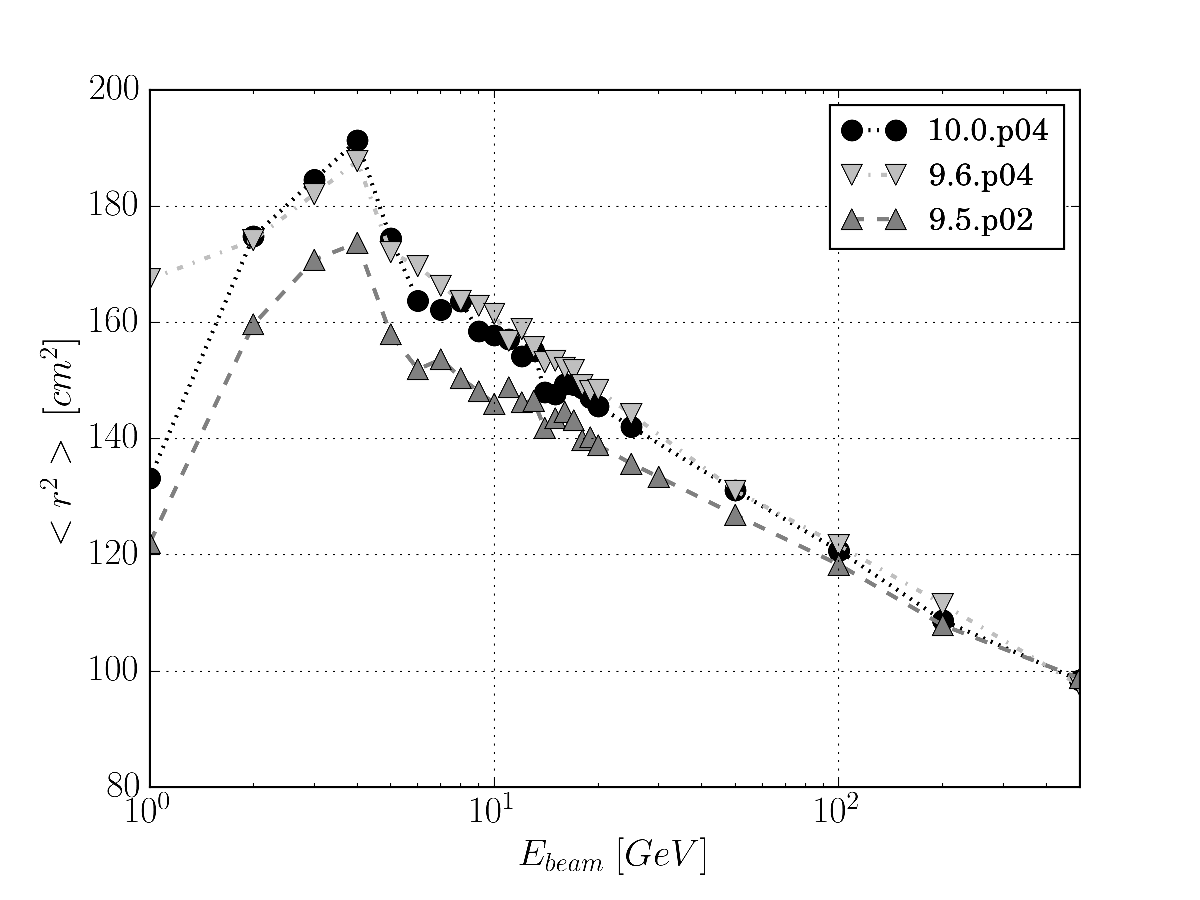
\includegraphics[width=0.5\textwidth]{figures/lateral.pdf}
    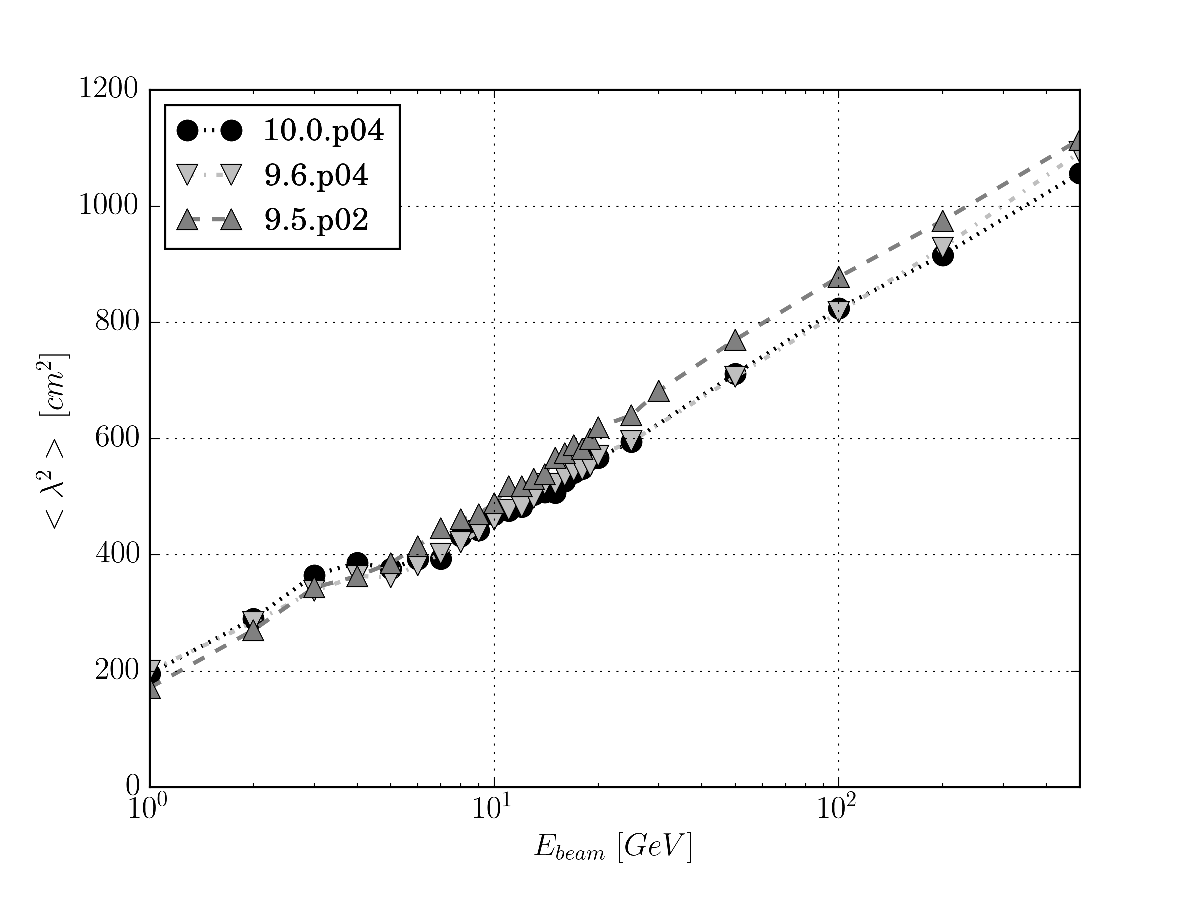
\includegraphics[width=0.5\textwidth]{figures/longitudinal.pdf}
   \caption{Comparison of recent \Gfour{} versions using the simplified
            iron/scintillator calorimeter (ATLAS TileCal).  Lateral 
            shower shapes (top) and longitudinal shower
            shapes (bottom) are shown.}
   \label{fig:shapes}
 \end{center}
\end{figure}

